\begin{frame}
	\begin{figure}[H]
		\centering
		\begin{minipage}[c][2cm][c]{0.3\textwidth}
			\begin{tikzpicture}[scale=0.5]
				\begin{axis}[
				anchor=east,  
				ticks=none,
				width=8cm,
				height=4cm,
				%ylabel=Iterações Lineares,
				xmin = 0,
				xmax = 0.04,
				ymin = 0,
				ymax = 0.02]
				\pgfplotstableread{../data/interface_01.dat} 
				\teff
				\addplot[color=blue,mark=none,smooth] table from \teff;
				\end{axis}			
			\end{tikzpicture}	
		\end{minipage}
		\begin{minipage}[c][2cm][c]{0.5\textwidth}
			$w(x) = \frac{b}{2}$
		\end{minipage}
		\begin{minipage}[c][2cm][c]{0.3\textwidth}
			\begin{tikzpicture}[scale=0.5]
			\begin{axis}[
			anchor=east,  
			ticks=none,
			width=8cm,
			height=4cm,
			%ylabel=Iterações Lineares,
			xmin = 0,
			xmax = 0.04,
			ymin = 0,
			ymax = 0.02]
			\pgfplotstableread{../data/interface_02.dat} 
			\teff
			\addplot[color=blue,mark=none,smooth] table from \teff;
			\end{axis}			
			\end{tikzpicture}	
		\end{minipage}
		\begin{minipage}[c][2cm][c]{0.5\textwidth}
			\begin{equation*}
				w(x) = \left\lbrace\begin{array}{ll}
				\frac{19bx^2}{8a^2}-\frac{7bx}{24a}+\frac{b}{2}, & 0 \le x < \frac{a}{3} \\
				-\frac{25bx^2}{8a^2}+\frac{27bx}{8a}-\frac{b}{9}, &  \frac{a}{3} \le x < \frac{2a}{3} \\ 
				\frac{bx^2}{8a^2}-\frac{23bx}{24a}+\frac{4b}{3}, &  \frac{2a}{3} \le x \le a
				\end{array}\right.
			\end{equation*}
		\end{minipage}
		\begin{minipage}[c][2cm][c]{0.3\textwidth}
			\begin{tikzpicture}[scale=0.5]
			\begin{axis}[
			anchor=east,  
			ticks=none,
			width=8cm,
			height=4cm,
			%ylabel=Iterações Lineares,
			xmin = 0,
			xmax = 0.04,
			ymin = 0,
			ymax = 0.02]
			\pgfplotstableread{../data/interface_03.dat} 
			\teff
			\addplot[color=blue,mark=none,smooth] table from \teff;
			\end{axis}			
			\end{tikzpicture}	
		\end{minipage}
		\begin{minipage}[c][2cm][c]{0.5\textwidth}
			$ w(x) = \frac{b}{2} + \frac{1}{20} \cos\frac{4 \pi  x}{a}$
		\end{minipage}
	\end{figure}
\end{frame}

\begin{frame}
	\begin{figure}[H]
		\centering
		\begin{minipage}[c][2cm][c]{0.3\textwidth}
			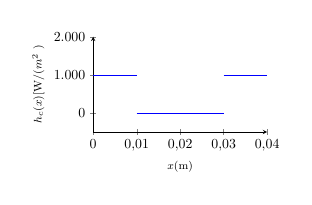
\begin{tikzpicture}[scale=0.5]
			\begin{axis}[
			/pgf/number format/1000 sep={.},/pgf/number format/use comma,
			axis lines=left,
			xmin = 0,
			xmax = 0.04,
			ymin = -500,
			ymax = 2000,
			restrict y to domain=-500:2000,
			scaled x ticks = false,
			scaled y ticks = false,
			x tick label style={/pgf/number format/fixed},
			y tick label style={/pgf/number format/fixed},
			anchor=east,  
			width=6cm,
			height=4cm,
			label style={font=\footnotesize},
			xlabel = $x$(m),
			ylabel= $h_c(x)[$W/($\text{m}^2$ \celsius)]]
			\addplot[color=blue,mark=none,smooth, domain=0:0.01] {1000};
			\addplot[color=blue,mark=none,smooth, domain=0.01:0.03] {0};
			\addplot[color=blue,mark=none,smooth, domain=0.03:0.04] {1000};
			\end{axis}			
			\end{tikzpicture}	
		\end{minipage}
		\begin{minipage}[c][2cm][c]{0.5\textwidth}
			\begin{equation*}
				h_c(x) = \left\lbrace
							\begin{array}{ll}
								h_{max}, & x < \frac{a}{4}, x > \frac{3a}{4} \\ 
								0 , & \frac{a}{4} < x < \frac{3a}{4}
							\end{array}
						\right.
			\end{equation*}
		\end{minipage}
		\begin{minipage}[c][2cm][c]{0.3\textwidth}
			\begin{tikzpicture}[scale=0.5]
			\begin{axis}[
			/pgf/number format/1000 sep={.},/pgf/number format/use comma,
			axis lines=left,
			xmin = 0,
			xmax = 0.04,
			ymin = -500,
			ymax = 2000,
			restrict y to domain=-500:2000,
			scaled x ticks = false,
			scaled y ticks = false,
			x tick label style={/pgf/number format/fixed},
			y tick label style={/pgf/number format/fixed},
			anchor=east,  
			width=6cm,
			height=4cm,
			label style={font=\footnotesize},
			xlabel = $x$(m),
			ylabel= $h_c(x)$[W/($\text{m}^2$ \celsius)]]
			\pgfplotstableread{../data/conductance_02.dat} 
			\teff
			\addplot[color=blue,mark=none,smooth] table from \teff;
			\end{axis}			
			\end{tikzpicture}	
		\end{minipage}
		\begin{minipage}[c][2cm][c]{0.5\textwidth}
			$h_c(x) = \sin\displaystyle\frac{\pi x}{a}$
		\end{minipage}
		\begin{minipage}[c][2cm][c]{0.3\textwidth}
			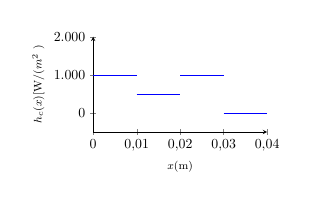
\begin{tikzpicture}[scale=0.5]
			\begin{axis}[
			/pgf/number format/1000 sep={.},/pgf/number format/use comma,
			axis lines=left,
			xmin = 0,
			xmax = 0.04,
			ymin = -500,
			ymax = 2000,
			restrict y to domain=-500:2000,
			scaled x ticks = false,
			scaled y ticks = false,
			x tick label style={/pgf/number format/fixed},
			y tick label style={/pgf/number format/fixed},
			anchor=east,  
			width=6cm,
			height=4cm,
			label style={font=\footnotesize},
			xlabel = $x$(m),
			ylabel= $h_c(x)$[W/($\text{m}^2$ \celsius)]]
			\addplot[color=blue,mark=none,smooth, domain=0:0.01] {1000};
			\addplot[color=blue,mark=none,smooth, domain=0.01:0.02] {500};
			\addplot[color=blue,mark=none,smooth, domain=0.02:0.03] {1000};
			\addplot[color=blue,mark=none,smooth, domain=0.03:0.04] {0};
			\end{axis}	
			\end{tikzpicture}	
		\end{minipage}
		\begin{minipage}[c][2cm][c]{0.5\textwidth}
			\begin{equation*}
			h_c(x) = \left\lbrace
			\begin{array}{ll}
				\displaystyle\frac{h_{max}}{2}, & x < \frac{a}{4}, \frac{a}{2} < x < \frac{3a}{4} \\
				h_{max}, & \frac{a}{4} < x < \frac{a}{2} \\
				0 , &x > \frac{3a}{4}
			\end{array}
			\right.
			\end{equation*}
		\end{minipage}
	\end{figure}
\end{frame}

\begin{frame}
	\frametitle{Salto de temperatura, interface 1}
	\begin{figure}[H]		
		\graficointerface{1}
		\graficoestimativa{delta_temperatura}{1}{1}{20}{06}{02}{a}{\Delta T\big|_{\Gamma}}{\celsius}
		\graficoestimativa{delta_temperatura}{1}{2}{20}{04}{04}{a}{\Delta T\big|_{\Gamma}}{\celsius}
		\graficoestimativa{delta_temperatura}{1}{3}{20}{06}{03}{a}{\Delta T\big|_{\Gamma}}{\celsius}
		\legendagraficos	
		\graficosctclegenda		
	\end{figure}
\end{frame}

\begin{frame}
	\frametitle{Fluxo de calor, interface 1}
	\begin{figure}[H]		
		\graficointerface{1}
		\graficoestimativa{fluxo_calor}{1}{1}{20}{06}{04}{a}{-k_1 \frac{\partial T_1}{\partial\mathbf{n}_1}\big|_{\Gamma}}{W/$\text{m}^2$}
		\graficoestimativa{fluxo_calor}{1}{2}{20}{04}{04}{a}{-k_1 \frac{\partial T_1}{\partial\mathbf{n}_1}\big|_{\Gamma}}{W/$\text{m}^2$}
		\graficoestimativa{fluxo_calor}{1}{3}{20}{06}{04}{a}{-k_1 \frac{\partial T_1}{\partial\mathbf{n}_1}\big|_{\Gamma}}{W/$\text{m}^2$}
		\legendagraficos
		\graficosctclegenda		
	\end{figure}
\end{frame}

\begin{frame}
	\frametitle{Condutância térmica de contato, interface 1}
	\begin{figure}[H]		
		\graficointerface{1}
		\graficoctc{02}{01}{1}{a}
		\graficoctc{02}{02}{2}{b}
		\graficoctc{02}{03}{3}{c}
		\legendagraficos
		%\graficosctclegenda		
	\end{figure}
\end{frame}

\begin{frame}
	\frametitle{Salto de temperatura, interface 2}
	\begin{figure}[H]		
		\graficointerface{2}
		\graficoestimativa{delta_temperatura}{2}{1}{20}{11}{09}{a}{\Delta T\big|_{\Gamma}}{\celsius}
		\graficoestimativa{delta_temperatura}{2}{2}{20}{09}{07}{a}{\Delta T\big|_{\Gamma}}{\celsius}
		\graficoestimativa{delta_temperatura}{2}{3}{20}{11}{09}{a}{\Delta T\big|_{\Gamma}}{\celsius}
		\legendagraficos	
		\graficosctclegenda		
	\end{figure}
\end{frame}

\begin{frame}
	\frametitle{Fluxo de calor, interface 2}
	\begin{figure}[H]		
		\graficointerface{2}
		\graficoestimativa{fluxo_calor}{2}{1}{20}{10}{06}{a}{-k_1 \frac{\partial T_1}{\partial\mathbf{n}_1}\big|_{\Gamma}}{W/$\text{m}^2$}
		\graficoestimativa{fluxo_calor}{2}{2}{20}{06}{06}{a}{-k_1 \frac{\partial T_1}{\partial\mathbf{n}_1}\big|_{\Gamma}}{W/$\text{m}^2$}
		\graficoestimativa{fluxo_calor}{2}{3}{19}{09}{04}{a}{-k_1 \frac{\partial T_1}{\partial\mathbf{n}_1}\big|_{\Gamma}}{W/$\text{m}^2$}
		\legendagraficos
		\graficosctclegenda		
	\end{figure}
\end{frame}

\begin{frame}
	\frametitle{Condutância térmica de contato, interface 2}
	\begin{figure}[H]		
		\graficointerface{2}
		\graficoctc{02}{01}{1}{a}
		\graficoctc{02}{02}{2}{b}
		\graficoctc{02}{03}{3}{c}
		\legendagraficos
		%\graficosctclegenda		
	\end{figure}
\end{frame}

\begin{frame}
	\frametitle{Salto de temperatura, interface 3}
	\begin{figure}[H]		
		\graficointerface{3}
		\graficoestimativa{delta_temperatura}{3}{1}{20}{08}{06}{a}{\Delta T\big|_{\Gamma}}{\celsius}
		\graficoestimativa{delta_temperatura}{3}{2}{20}{06}{04}{a}{\Delta T\big|_{\Gamma}}{\celsius}
		\graficoestimativa{delta_temperatura}{3}{3}{20}{08}{06}{a}{\Delta T\big|_{\Gamma}}{\celsius}
		\legendagraficos	
		\graficosctclegenda		
	\end{figure}
\end{frame}

\begin{frame}
	\frametitle{Fluxo de calor, interface 3}
	\begin{figure}[H]		
		\graficointerface{3}
		\graficoestimativa{fluxo_calor}{3}{1}{20}{06}{06}{a}{-k_1 \frac{\partial T_1}{\partial\mathbf{n}_1}\big|_{\Gamma}}{W/$\text{m}^2$}
		\graficoestimativa{fluxo_calor}{3}{2}{20}{04}{04}{a}{-k_1 \frac{\partial T_1}{\partial\mathbf{n}_1}\big|_{\Gamma}}{W/$\text{m}^2$}
		\graficoestimativa{fluxo_calor}{3}{3}{20}{06}{03}{a}{-k_1 \frac{\partial T_1}{\partial\mathbf{n}_1}\big|_{\Gamma}}{W/$\text{m}^2$}
		\legendagraficos
		\graficosctclegenda		
	\end{figure}
\end{frame}

\begin{frame}
	\frametitle{Condutância térmica de contato, interface 3}
	\begin{figure}[H]		
		\graficointerface{3}
		\graficoctc{03}{01}{1}{a}
		\graficoctc{03}{02}{2}{b}
		\graficoctc{03}{03}{3}{c}
		\legendagraficos
		%\graficosctclegenda		
	\end{figure}
\end{frame}